% Options for packages loaded elsewhere
\PassOptionsToPackage{unicode}{hyperref}
\PassOptionsToPackage{hyphens}{url}
%
\documentclass[
]{article}
\usepackage{amsmath,amssymb}
\usepackage{iftex}
\ifPDFTeX
  \usepackage[T1]{fontenc}
  \usepackage[utf8]{inputenc}
  \usepackage{textcomp} % provide euro and other symbols
\else % if luatex or xetex
  \usepackage{unicode-math} % this also loads fontspec
  \defaultfontfeatures{Scale=MatchLowercase}
  \defaultfontfeatures[\rmfamily]{Ligatures=TeX,Scale=1}
\fi
\usepackage{lmodern}
\ifPDFTeX\else
  % xetex/luatex font selection
\fi
% Use upquote if available, for straight quotes in verbatim environments
\IfFileExists{upquote.sty}{\usepackage{upquote}}{}
\IfFileExists{microtype.sty}{% use microtype if available
  \usepackage[]{microtype}
  \UseMicrotypeSet[protrusion]{basicmath} % disable protrusion for tt fonts
}{}
\makeatletter
\@ifundefined{KOMAClassName}{% if non-KOMA class
  \IfFileExists{parskip.sty}{%
    \usepackage{parskip}
  }{% else
    \setlength{\parindent}{0pt}
    \setlength{\parskip}{6pt plus 2pt minus 1pt}}
}{% if KOMA class
  \KOMAoptions{parskip=half}}
\makeatother
\usepackage{xcolor}
\usepackage[margin=1in]{geometry}
\usepackage{graphicx}
\makeatletter
\def\maxwidth{\ifdim\Gin@nat@width>\linewidth\linewidth\else\Gin@nat@width\fi}
\def\maxheight{\ifdim\Gin@nat@height>\textheight\textheight\else\Gin@nat@height\fi}
\makeatother
% Scale images if necessary, so that they will not overflow the page
% margins by default, and it is still possible to overwrite the defaults
% using explicit options in \includegraphics[width, height, ...]{}
\setkeys{Gin}{width=\maxwidth,height=\maxheight,keepaspectratio}
% Set default figure placement to htbp
\makeatletter
\def\fps@figure{htbp}
\makeatother
\setlength{\emergencystretch}{3em} % prevent overfull lines
\providecommand{\tightlist}{%
  \setlength{\itemsep}{0pt}\setlength{\parskip}{0pt}}
\setcounter{secnumdepth}{-\maxdimen} % remove section numbering
\ifLuaTeX
  \usepackage{selnolig}  % disable illegal ligatures
\fi
\IfFileExists{bookmark.sty}{\usepackage{bookmark}}{\usepackage{hyperref}}
\IfFileExists{xurl.sty}{\usepackage{xurl}}{} % add URL line breaks if available
\urlstyle{same}
\hypersetup{
  pdftitle={Question5},
  hidelinks,
  pdfcreator={LaTeX via pandoc}}

\title{Question5}
\author{}
\date{\vspace{-2.5em}2025-06-18}

\begin{document}
\maketitle

\hypertarget{can-we-identify-global-patterns-in-agricultural-performance-and-energy-water-usage-among-countries}{%
\section{Can we identify global patterns in agricultural performance and
energy-water usage among countries
?}\label{can-we-identify-global-patterns-in-agricultural-performance-and-energy-water-usage-among-countries}}

\hypertarget{data-exploration}{%
\section{data exploration}\label{data-exploration}}

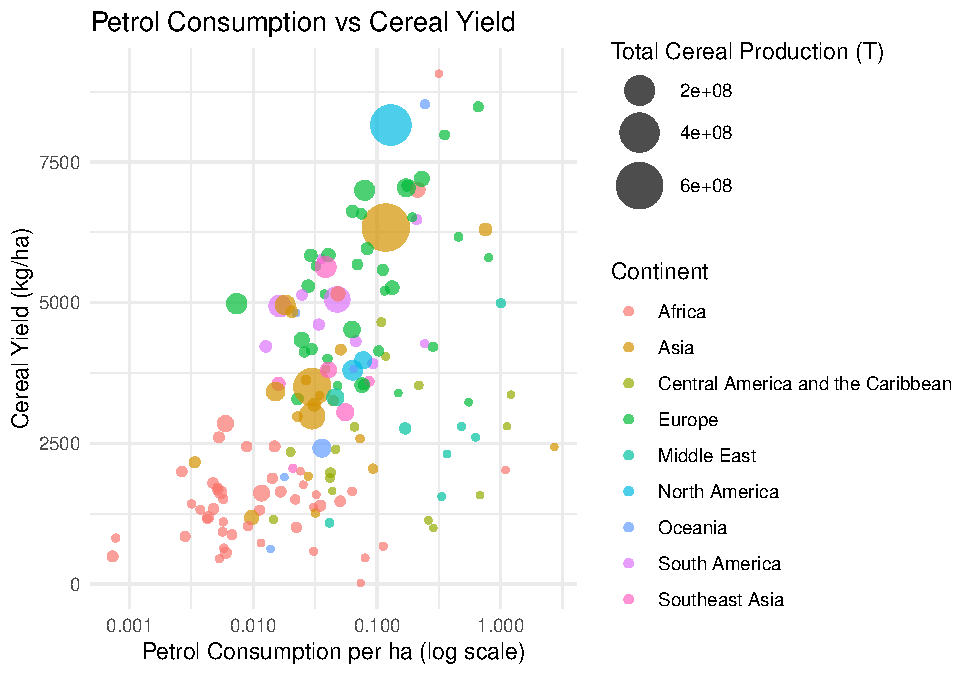
\includegraphics{Question5_files/figure-latex/unnamed-chunk-2-1.pdf}

This first plot suggests a potential positive correlation between petrol
consumption per hectare and cereal yield. Additionally, countries with
higher total cereal production (indicated by the size of the points)
also tend to exhibit higher petrol usage and yield levels. We can also
observe clusters by continent, suggesting similarities within the same
continent.

A plausible hypothesis emerging from this visualization is that
countries with higher energy inputs may achieve more productive
agricultural systems.


\includegraphics{Question5_files/figure-latex/unnamed-chunk-3-1.pdf}

These box plots represent the distribution of cereal yields (in orange)
and the distribution of water consumption (in blue) for all continents.
These values have been normalized between 0 and 1 for comparison
purposes.

From an agronomic point of view, cereals are very water-intensive crops,
and agriculture is one of the activities that exploits this resource the
most. This graph seems to show a slight correlation between these two
parameters. However, in Africa, the opposite situation can be observed.
This graph seems to confirm agronomic knowledge by suggesting that a
country's water consumption enables it to increase its cereal yields.

However, we cannot rule out a confounding variable. For example, we can
imagine that developed countries have a rich economy, partly produced by
strong agriculture. These same countries have developed water supply
systems for industry and residents.

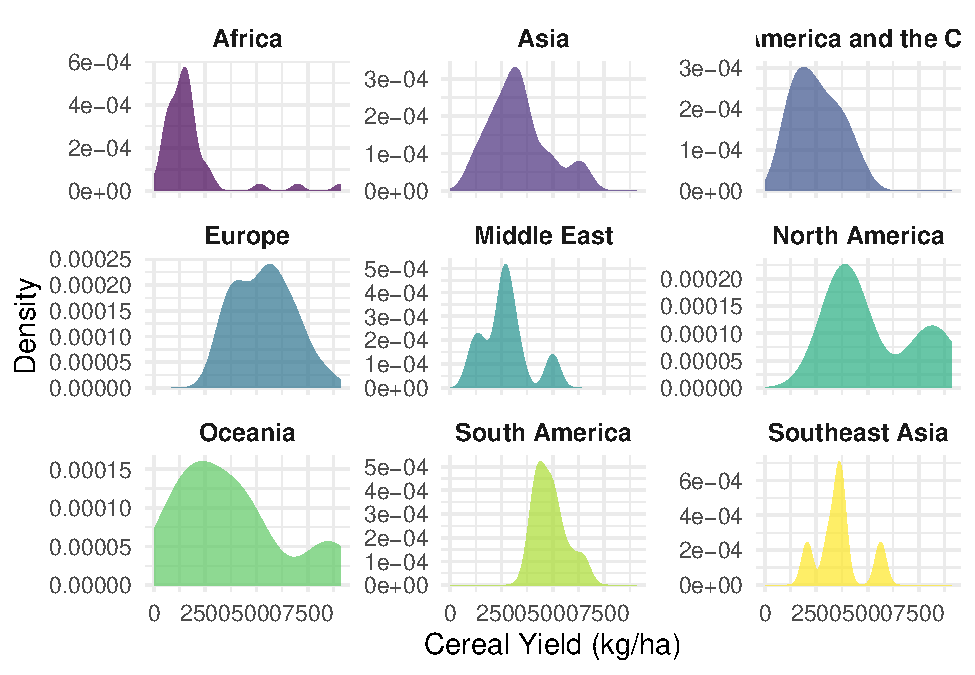
\includegraphics{Question5_files/figure-latex/unnamed-chunk-4-1.pdf}

This graph also shows the distribution of cereal yields for each
continent, but in a more detailed way by showing its distribution.

It allows us to see significant differences in productivity between
continents. Africa appears to be the least productive, while Europe and
North America are the most productive. The study of modes allows us to
observe continental within differences. For example, European yields do
not show a clear mode, suggesting uniformity of production between
European countries. In Southeast Asia, there appear to be three yield
groups. For North America, consisting solely of Canada and the United
States, these two modes are clearly observable.

\hypertarget{principal-component-analysis-pca}{%
\section{Principal Component Analysis
(PCA)}\label{principal-component-analysis-pca}}

In this analysis, we performed a Principal Component Analysis (PCA) on a
set of standardized (per hectare of arable land) agricultural,
environmental, and input-related variables across countries. T he
variables include several yield measures (e.g., cereal, maize, fruit,
pulses, sugar crops), energy consumption per hectare (coal, petrol,
natural gas), agricultural water withdrawal per hectare, fertilizer
input (NPK, herbicides, insecticides), agricultural production value per
hectare, and the share of irrigated cropland.

These variables were grouped into thematic categories---Yield, Energy,
Fertilizer, Water, Agricultural Structure, Value, and Production---to
better understand the multidimensional structure of agricultural
efficiency and resource use across countries.


\includegraphics{Question5_files/figure-latex/unnamed-chunk-7-1.pdf}

The scree plot below shows the percentage of total variance explained by
each principal component. The first two principal components explain
approximately 33\% and 13\% of the variance, respectively, accounting
for nearly 46\% of the total variability.

While the elbow in the scree plot is not very pronounced (with a slight
inflection point after the first component), we proceed by focusing on
the first two dimensions to explore the main patterns in the data.

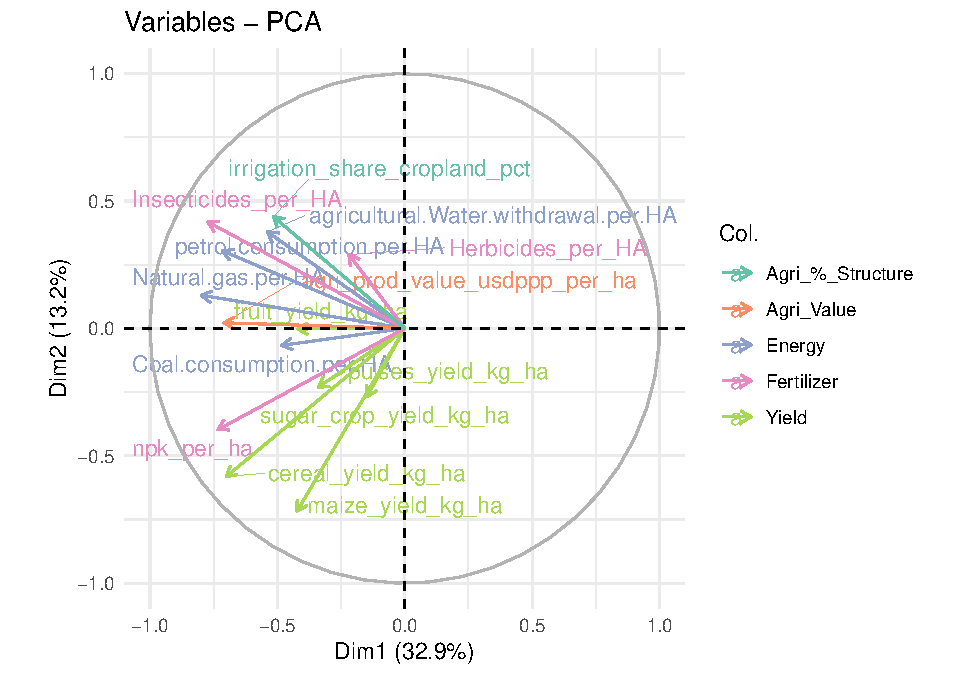
\includegraphics{Question5_files/figure-latex/unnamed-chunk-8-1.pdf}

This plot shows how each variable contributes to the two main principal
components. The direction and length of each arrow represent the
contribution and correlation of the variable with the components.

Variables related to agricultural yields cluster in the bottom-left
quadrant, suggesting they contribute strongly to Dimension 2. In
contrast, variables associated with energy consumption (coal, petrol,
gas) are mostly orthogonal to the yield variables and point toward the
upper-left quadrant, indicating a strong contribution to Dimension 1.
This suggests that yield and energy consumption are not strongly
correlated in this dataset.

Similarly, most input-related variables (insecticides, herbicides) align
with energy variables, with the exception of NPK fertilizers, which
point in the same direction as the yield variables. This may indicate
that NPK use is more closely associated with crop productivity than
other inputs.

Interestingly, water consumption variables align with energy usage
rather than with yields, suggesting that higher water withdrawal does
not necessarily translate into higher agricultural performance at a
global scale.

The variable representing the average agricultural production value per
hectare (USD PPP) points in an intermediate direction. A reasonable
interpretation is that energy consumption is more reflective of general
development level (e.g., high energy use in oil-exporting countries with
low crop yields), rather than of agricultural performance. In contrast,
countries with developed agricultural systems and access to irrigation
might achieve both higher yield and higher value-added production per
hectare. Hence, the average production value captures both productivity
and the diversity of economically valuable crops.

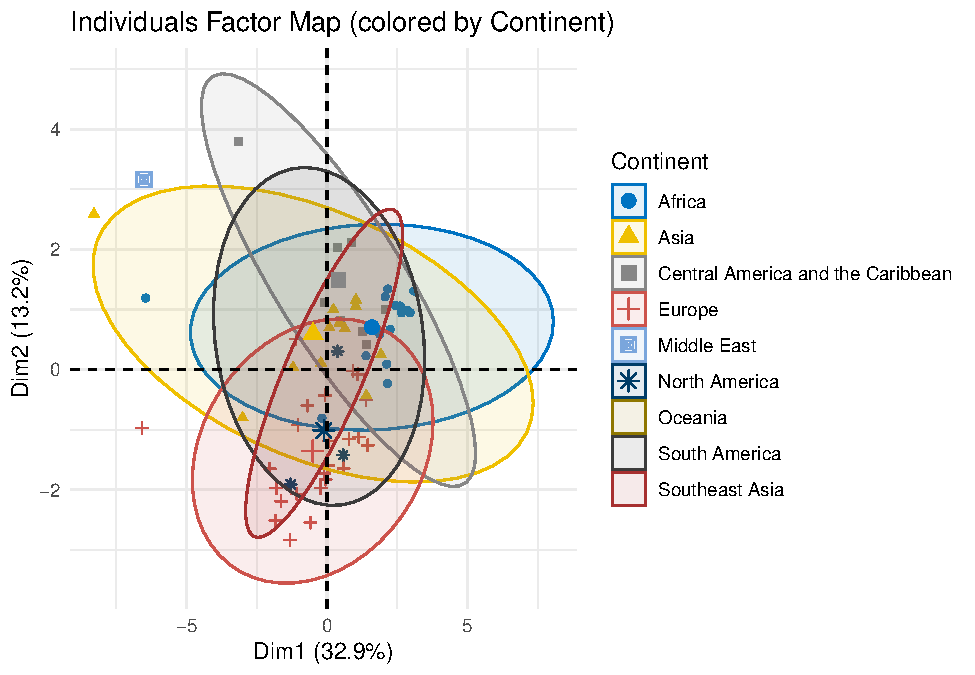
\includegraphics{Question5_files/figure-latex/unnamed-chunk-9-1.pdf}
\#\#\# Bottom-left quadrant (−Dim1, −Dim2): Characterized by high
agricultural yields, intensive NPK fertilizer use, and moderate to lower
energy/water consumption.

Dominated by European and Southeast Asian countries.

This quadrant may represent efficient and productive agricultural
systems, where outputs are achieved with relatively optimized input use.

\hypertarget{upper-left-quadrant-dim1-dim2}{%
\subsubsection{Upper-left quadrant (−Dim1,
+Dim2):}\label{upper-left-quadrant-dim1-dim2}}

Associated with high energy and water consumption, but lower
agricultural yields.

Includes some countries from North America and Oceania.

This could reflect input-heavy systems with lower overall efficiency or
different agricultural priorities (e.g., livestock over crops).

\hypertarget{right-side-of-the-map-dim1}{%
\subsubsection{Right side of the map
(+Dim1):}\label{right-side-of-the-map-dim1}}

Countries in this region exhibit lower energy and water use, though
their yield or input profiles are more mixed.

Several African and Asian countries cluster here.

This may reflect less resource-intensive agriculture, either due to
structural constraints or different development levels.

\hypertarget{center-of-the-map}{%
\subsubsection{Center of the map:}\label{center-of-the-map}}

Countries from Central America, the Middle East, and others are
dispersed around the origin, indicating no strong association with
either axis. These may represent diverse or transitional profiles,
balancing input use and productivity.

\hypertarget{agricultural-value-per-hectare-a-crosscutting-variable}{%
\subsubsection{Agricultural Value per Hectare: A Crosscutting
Variable}\label{agricultural-value-per-hectare-a-crosscutting-variable}}

The variable representing the average agricultural production value per
hectare (USD PPP) appears to point in an intermediate
direction---neither fully aligned with input intensity nor with yield
exclusively. This suggests that:

Value creation may result from a combination of yield and input
optimization, rather than from raw input intensity alone.

Countries with both moderate yields and access to water/energy
infrastructure (e.g., some European nations) may achieve better economic
valorization of their land.

\hypertarget{caution-and-final-remarks}{%
\subsubsection{Caution and Final
Remarks}\label{caution-and-final-remarks}}

While the PCA helps differentiate agricultural input-output profiles,
several caveats apply:

Energy and water consumption do not directly correlate with higher
performance globally; contextual factors (e.g., climate, technology,
export orientation) likely moderate these effects.

The overlap of countries from different continents indicates high
internal heterogeneity, suggesting that development models and
agricultural strategies vary widely within regions.

Lastly, the PCA simplifies multidimensional relationships into two
axes---so non-linearities or interaction effects may be obscured.

\end{document}
